\begin{figure}[htp] \centering
    \begin{subfigure}
        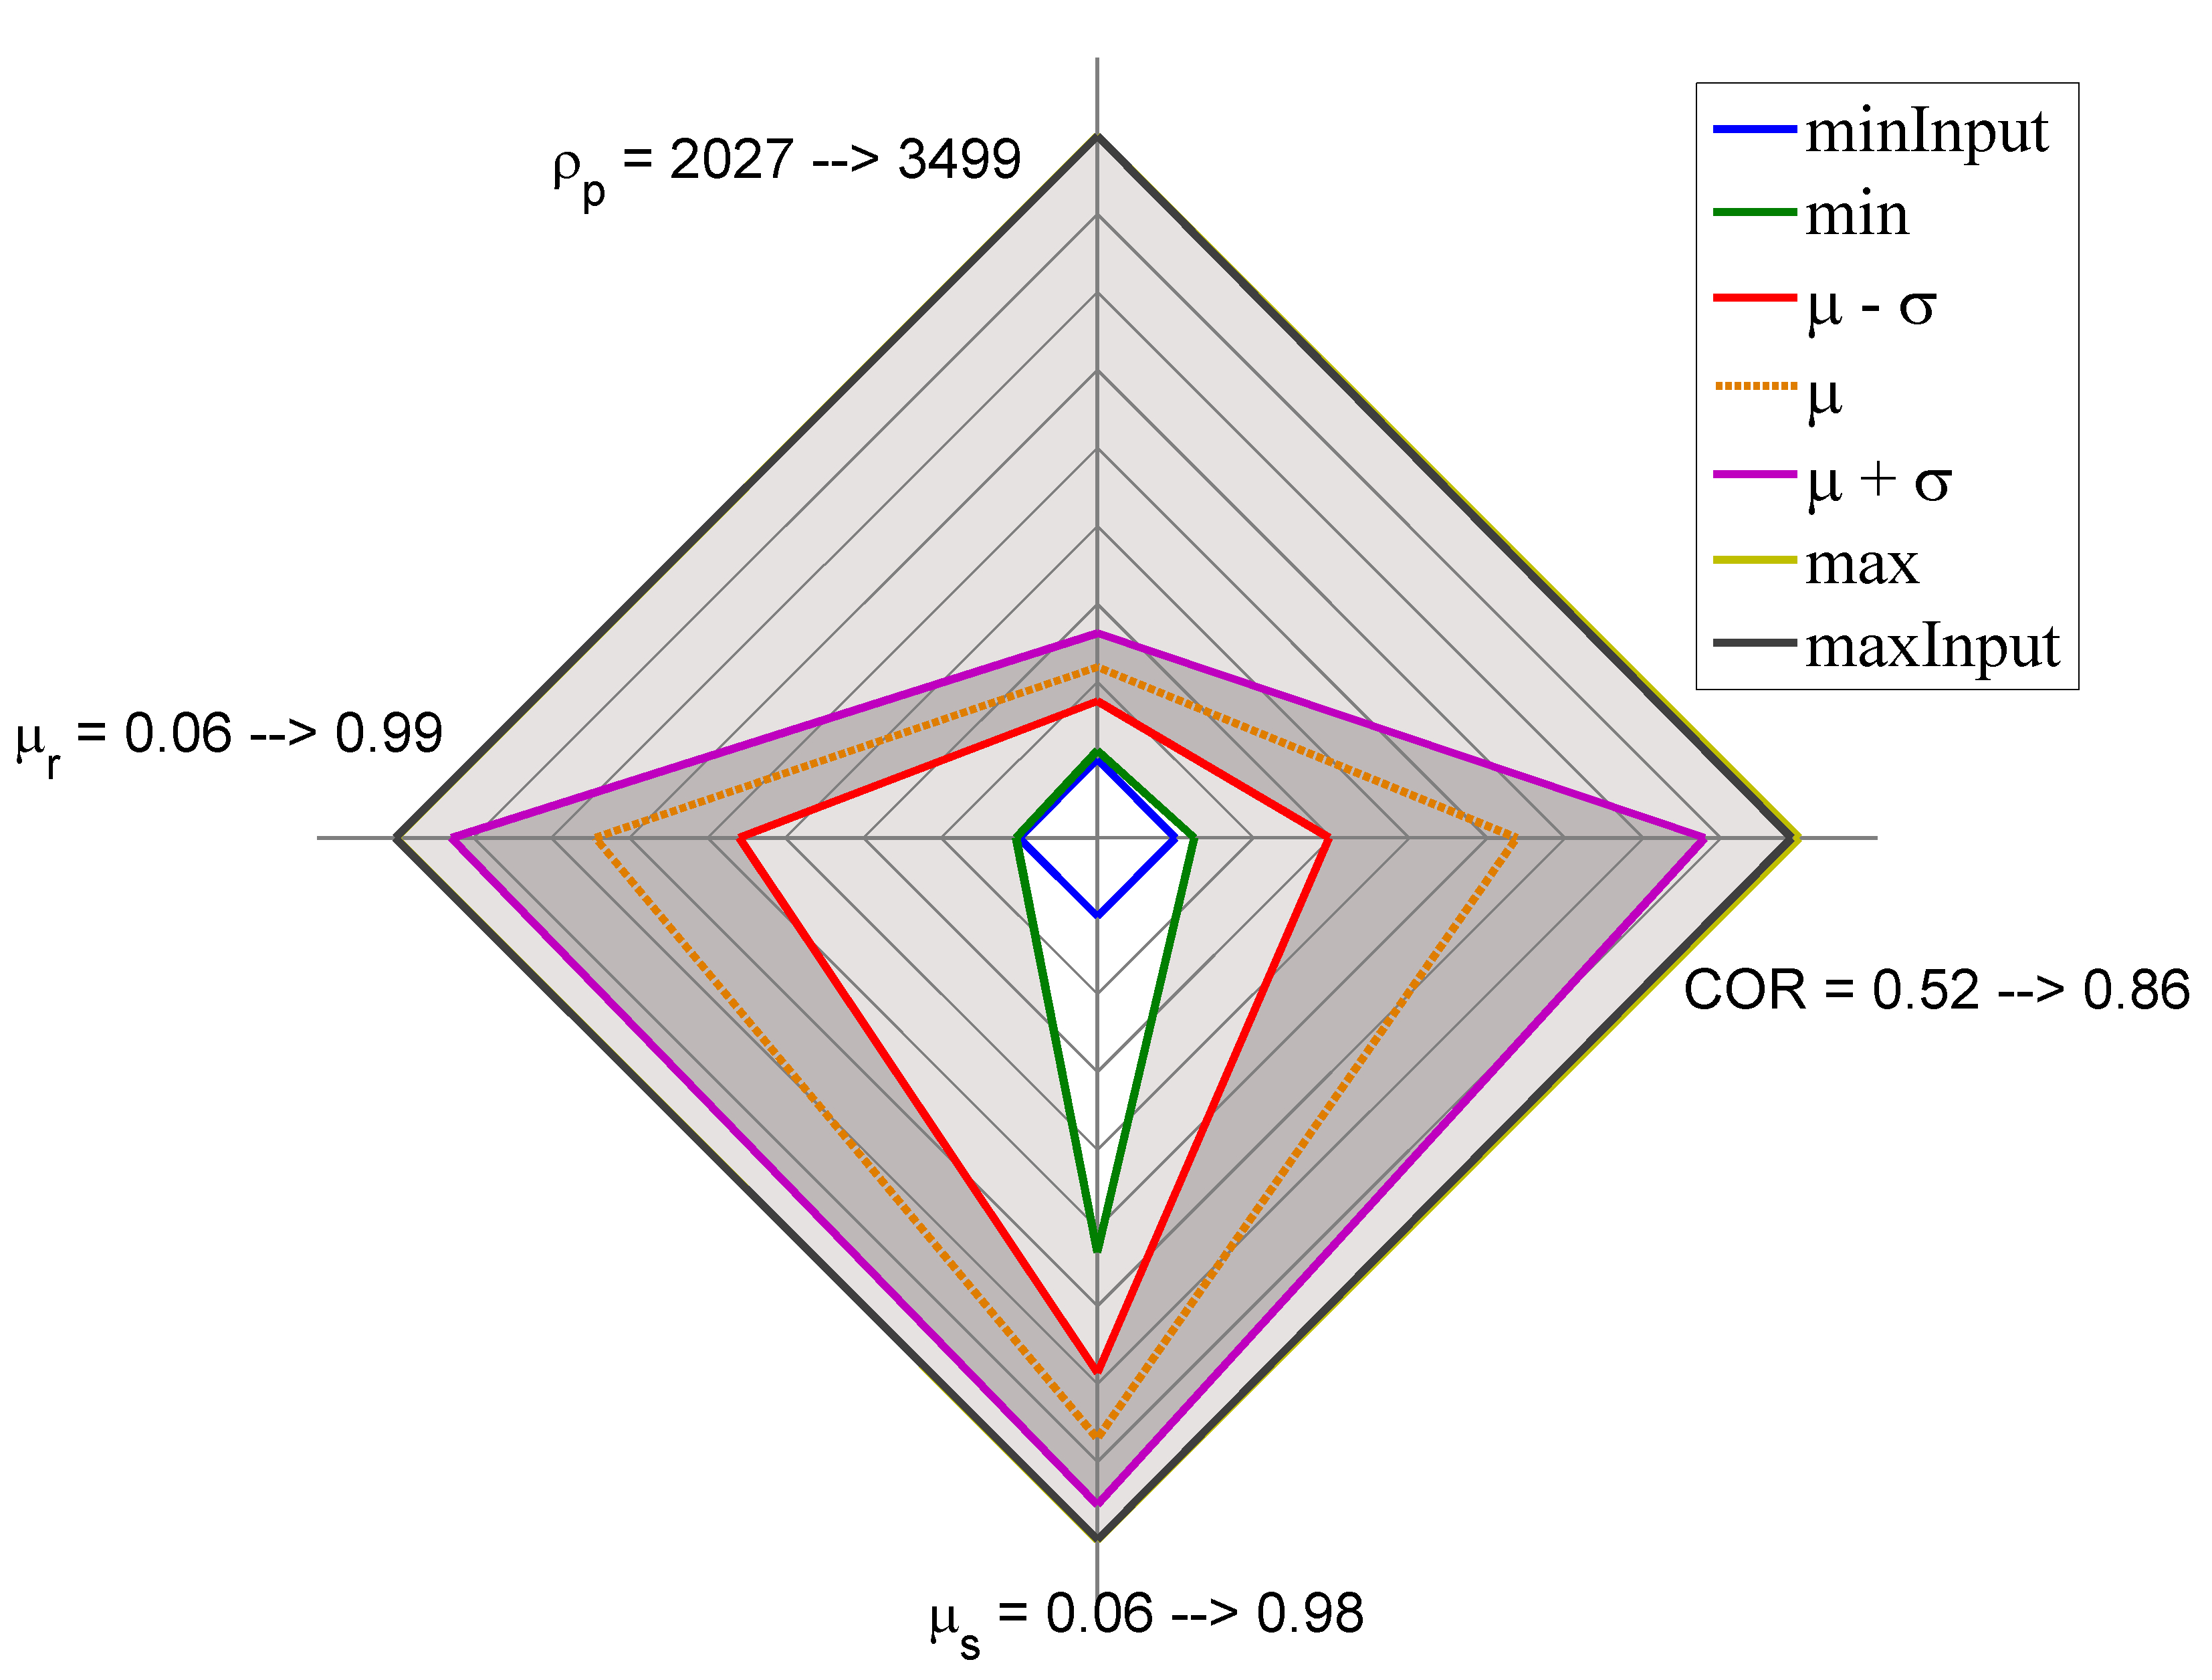
\includegraphics[width=0.5\textwidth]{images/original/24radarpirker1schulze10070}
        \caption{Radar plot, $SCT$, $\sigma_n=10070 ~[Pa]$, $P=1.0$}
        \label{fig:24radarpirker1schulze10070}
    \end{subfigure} \\
        \begin{subfigure}
        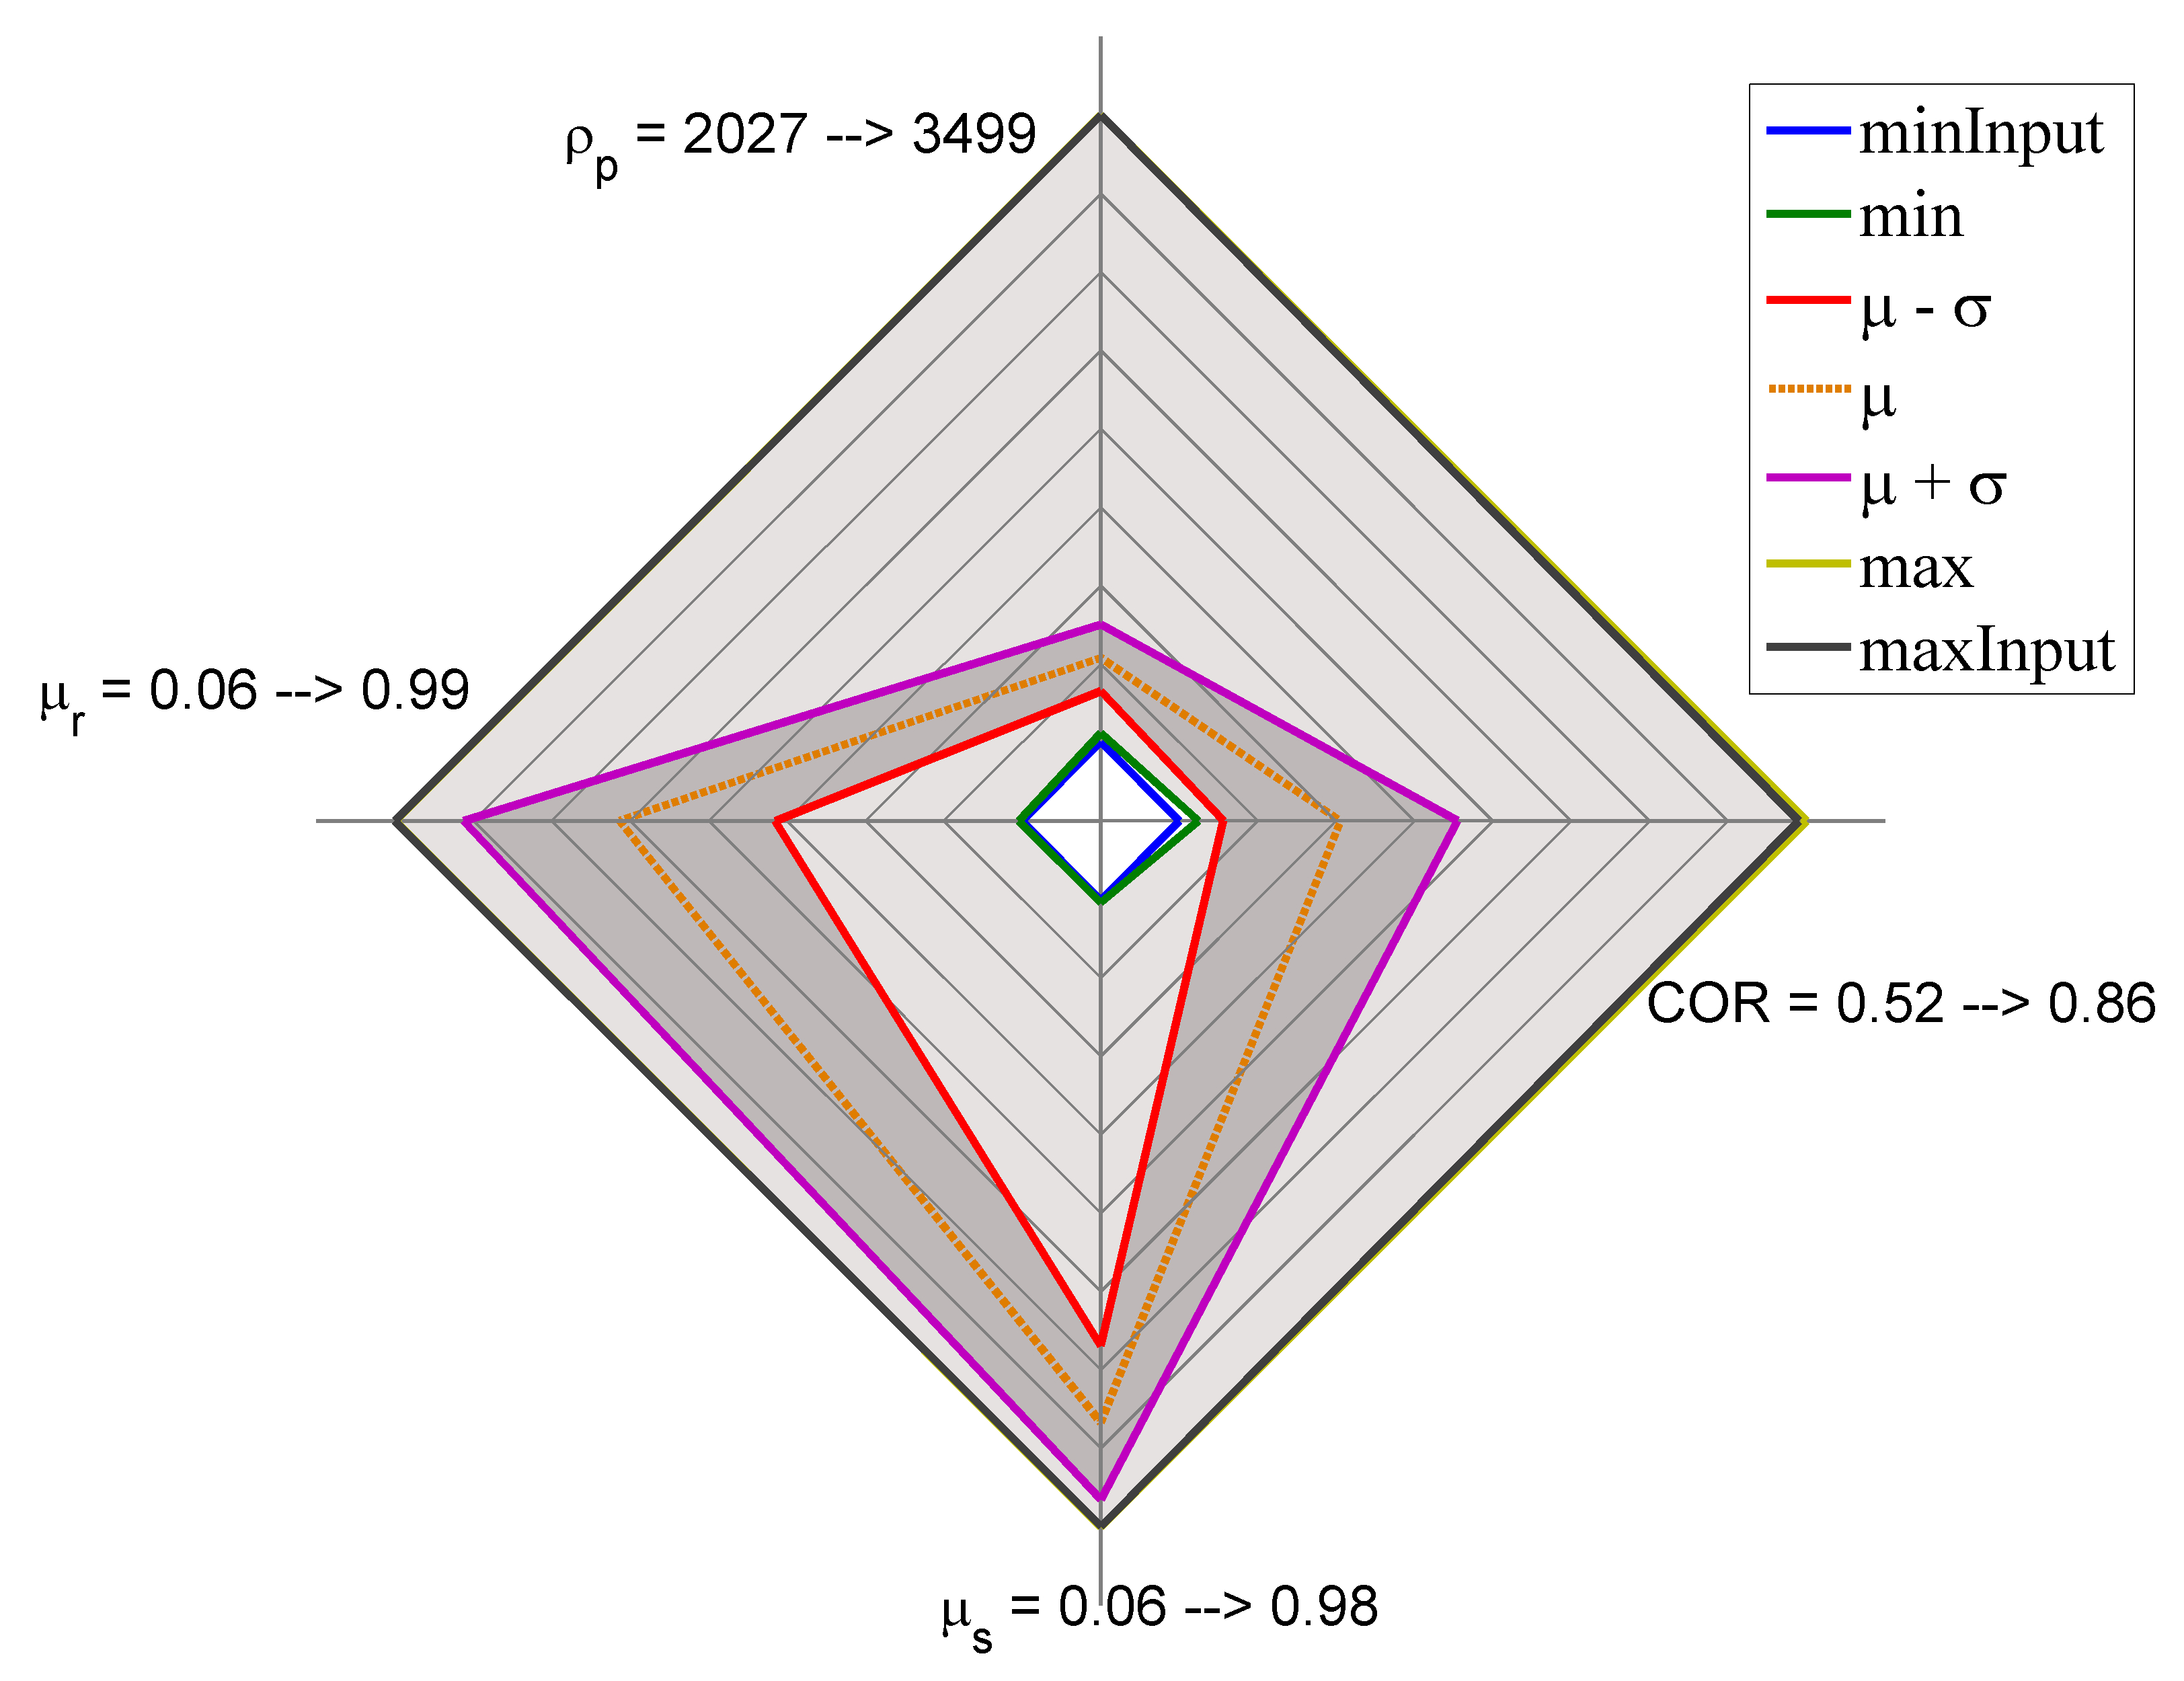
\includegraphics[width=0.5\columnwidth]{images/original/26radarpirker08schulze10070}
        \caption{Radar plot, $SCT$, $\sigma_n=10070 ~[Pa]$, $P=0.8$}
        \label{fig:26radarpirker08schulze10070} 
    \end{subfigure}\\
        \begin{subfigure}
        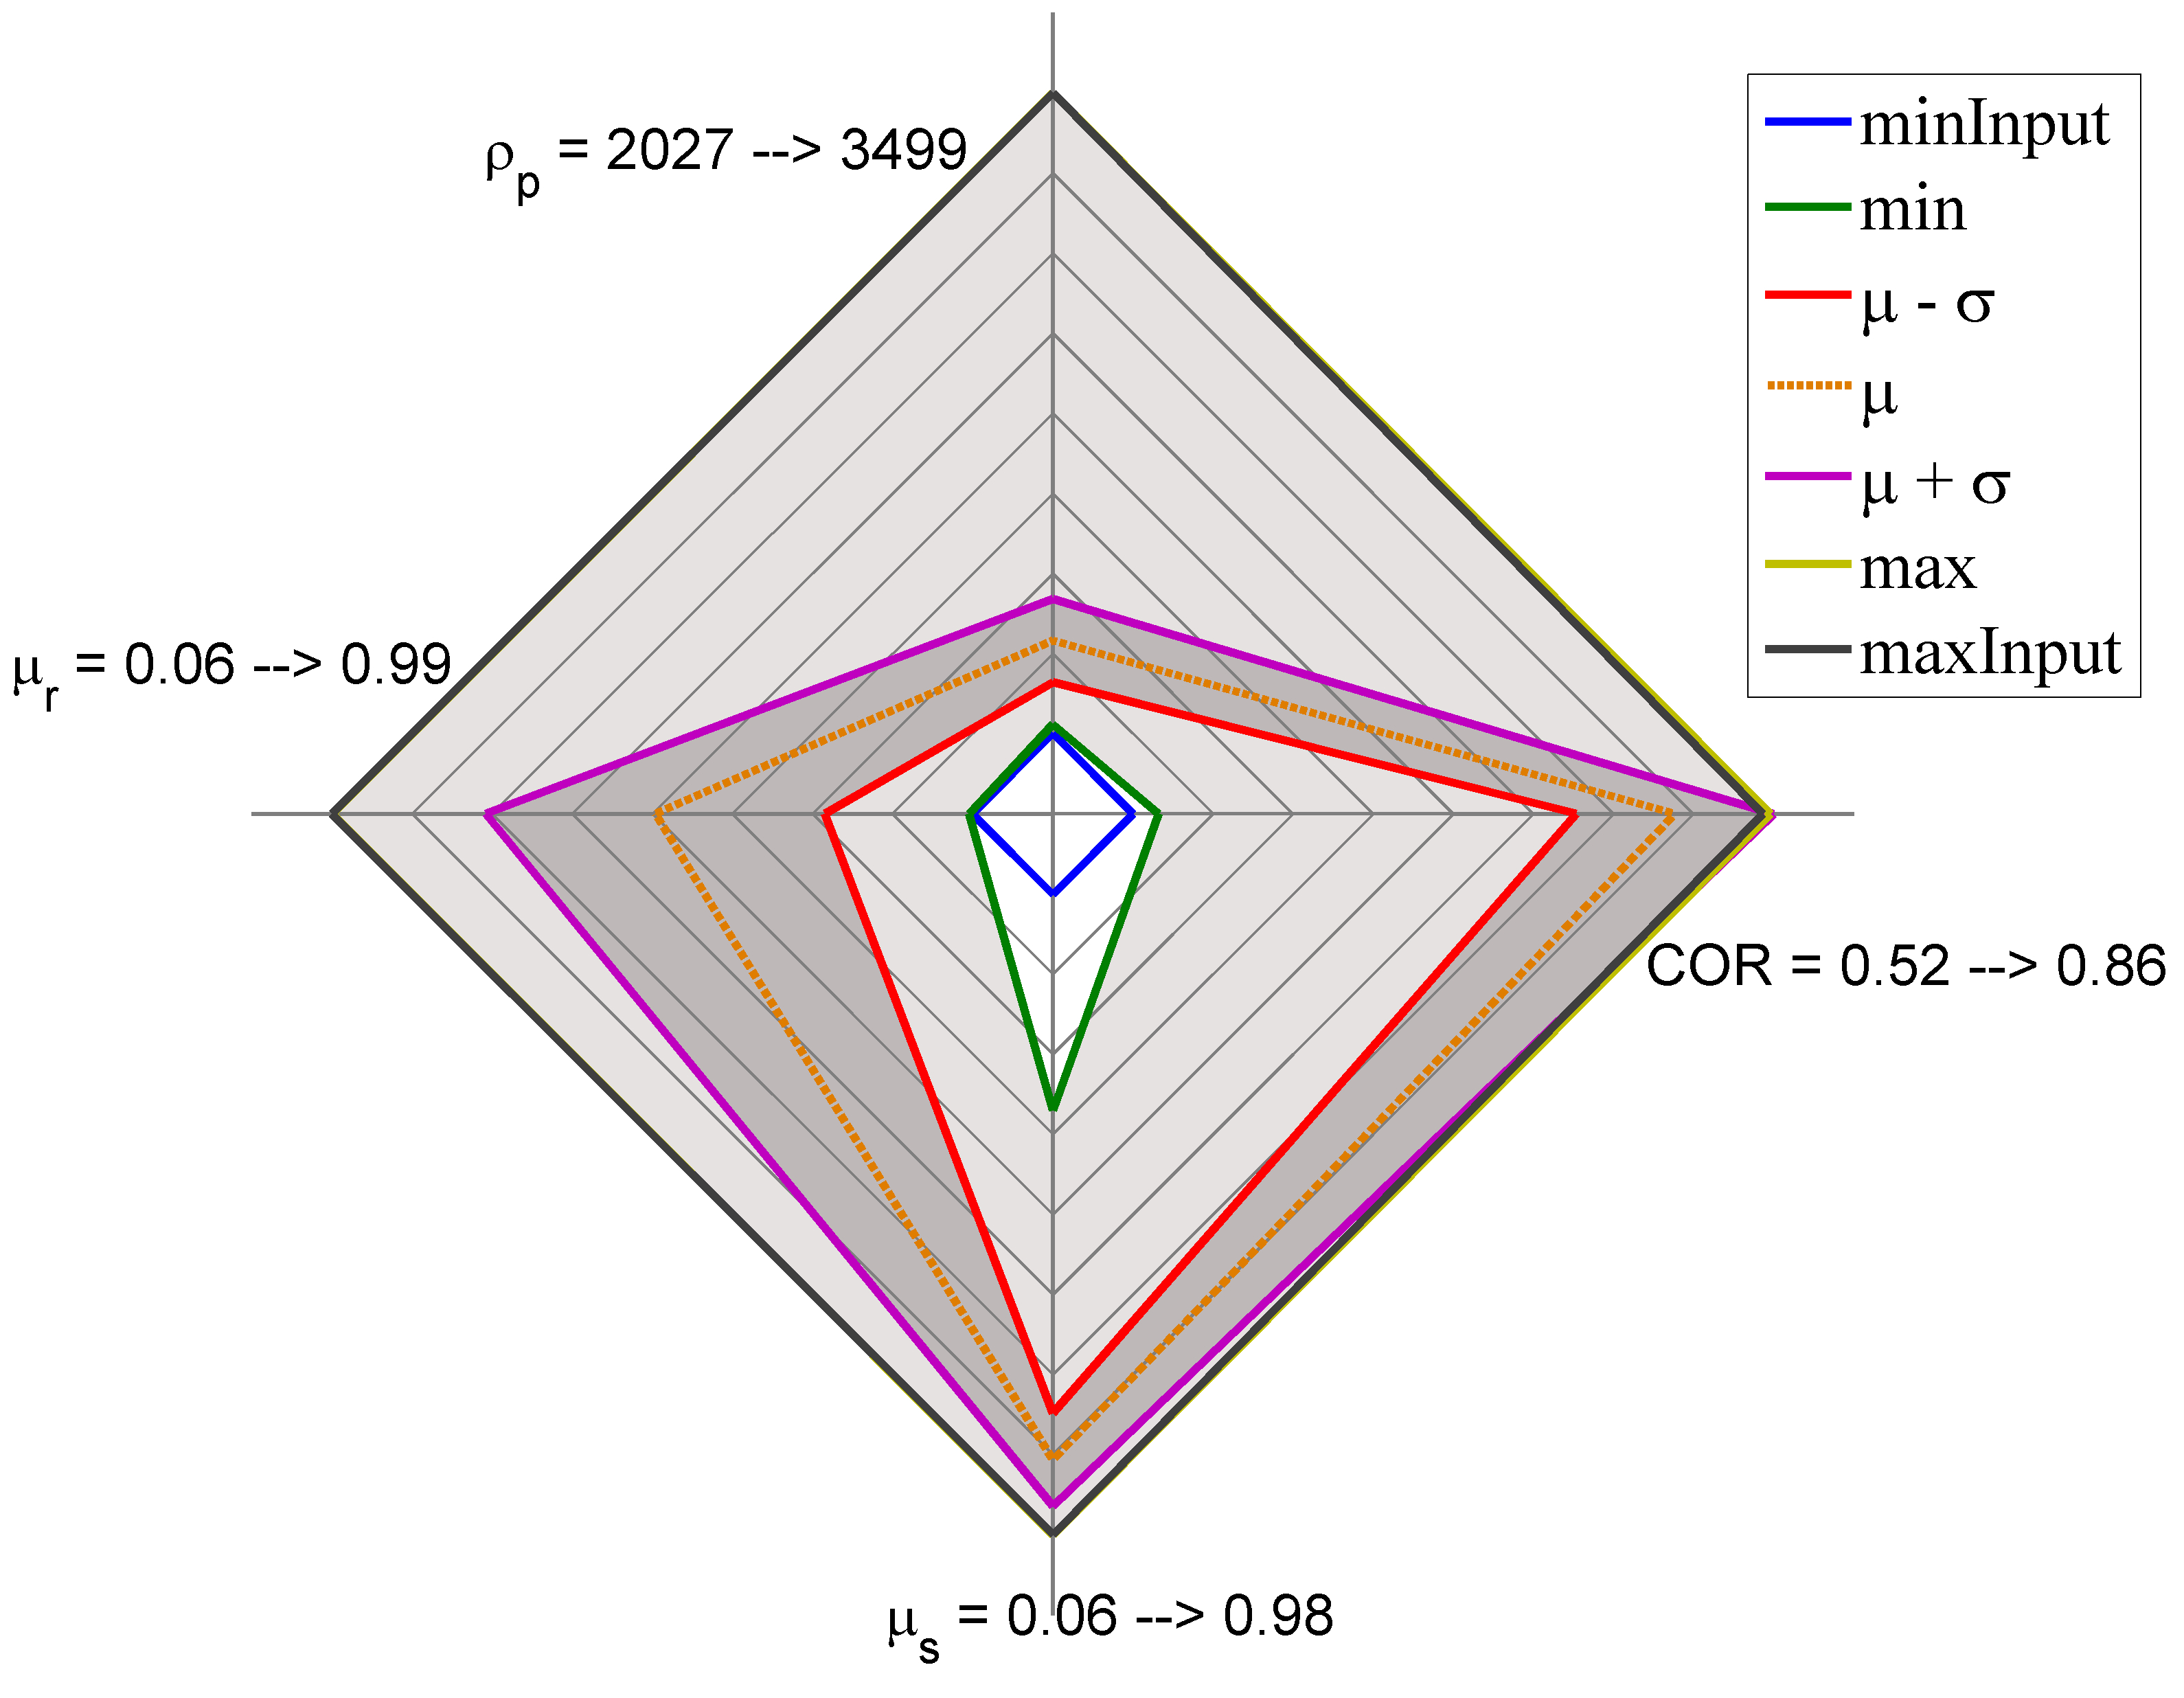
\includegraphics[width=0.5\columnwidth]{images/original/28radarpirker12schulze10070}
        \caption{Radar plot, $SCT$, $\sigma_n=10070 ~[Pa]$, $P=1.2$}
        \label{fig:28radarpirker12schulze10070} 
    \end{subfigure}
    \caption[Radar plot of valid simulations parameters for three different
    bulk behaviours measured by SCT]{Radar plot of valid simulations parameters for three different
    bulk behaviours measured by shear cell tester ($SCT$).
    Each axes of the radar plot represents one simulation parameters.
    Furthermore, the shaded area represents valid parameters combinations.
    Dark shaded values stand for the confidence range.
    We represent the tabbed combinations for one load condition of the shear cell. 
    Further explanation in the text.
   }
    \label{fig:29schulzeradarandcloud}
\end{figure}
% 
% The minimum and maximum values, together with the mean and the confidence range,
% provided by the square deviation, are shown.
%     Here, the values plotted are selected between the numerical
%     values from the $NN$ with initially the original experimental results for the shear cell tester $P=1.0$ (Fig.
%     \ref{fig:24radarpirker1schulze10070}). 
%     The confidence range is large, especially for the $COR$.
%     Instead, both the $\rho_p$  and the $\mu_s$ show a narrow confidence range. 
%     Later, they have been chosen with  
%     the virtual decreased results $P=0.8$
%     (\ref{fig:26radarpirker08schulze10070}).
%     The confidence range is narrower compared to $P=1.0$
%     The last image (Fig. \ref{fig:28radarpirker12schulze10070}) represents
%     instead the selection with the the virtual increased results $P=1.2$.
%     The plot shows a largely different confidence range. 